\input{preamble-libroTrabajoGrado3-Minimal.tex}
%% Title page information for article
\title{PROTOTIPO: Matemáticas IM\textsuperscript{\textregistered}\\
{\large Grado 3 - Unidad 4}\\[1ex]{\Huge Libro de trabajo}}
\author{Adaptación del Grupo LEMA\\
\href{https://www.grupolema.org}{\nolinkurl{https://www.grupolema.org}}
}

% Macro to store all cutout pages
\newcommand{\cutoutpages}{}

% Define cutoutpage environment with an optional argument for the footer
\NewDocumentEnvironment{cutoutpage}{O{}+b} % O{} = optional argument, +b = block
  {
    % Append cutout page content with a footer customization command
    \gappto\cutoutpages{%
      \cleardoublepage
      \fancypagestyle{cutoutstyle}{% Define a temporary style
        \fancyfoot[C]{#1} % Use the provided footer text
      }
      \thispagestyle{cutoutstyle} % Apply the new footer style
      #2\par % Content of the cutout page
    }
  }
  {}

% Append all stored cutout pages at the end of the document
\AfterEndDocument{%
  \vspace*{8cm}
  {\Huge HOJAS PARA RECORTAR}
  \cleardoublepage
  \cutoutpages
  \cleardoublepage
}



\date{Enero 16, 2025}
\begin{document}
%% bottom alignment is explicit, since it normally depends on oneside, twoside
\raggedbottom
%% Target for xref to top-level element is document start
\label{gra3-uni4}\hypertarget{gra3-uni4}{}
\maketitle
\thispagestyle{empty}
\cleardoublepage
%
%
\typeout{************************************************}
\typeout{Sección  Sección A -~¿Qué es la división?}
\typeout{************************************************}
%
\begin{sectionptx}{Sección}{Sección A -~¿Qué es la división?}{}{Sección A -~¿Qué es la división?}{}{}{gra3-uni4-secA}
%
%

\typeout{************************************************}
\typeout{Subsección  Lección 5 -~Escribamos expresiones de división}
\typeout{************************************************}
%
\begin{subsectionptx}{Subsección}{Lección 5 -~Escribamos expresiones de división}{}{Lección 5}{}{}{lec-escribamosExpresionesDivision}
%
%
\typeout{************************************************}
\typeout{Subsubsección  Actividad 1}
\typeout{************************************************}
%
% \cleardoublepage
\begin{cutoutpage}
\begin{subsubsectionptx}{Subsubsección}{Actividad 1}{}{Actividad 1}{}{}{lec-escribamosExpresionesDivision-act1}
\begin{activity}{Actividad}{Clasificación de tarjetas: Todo sobre bichos.}{act-clasificacionDeTarjetas-todoSobreBichos}%
Tarjetas para recortar:%
\end{activity}%
% \begin{image}{0}{1}{0}{}%
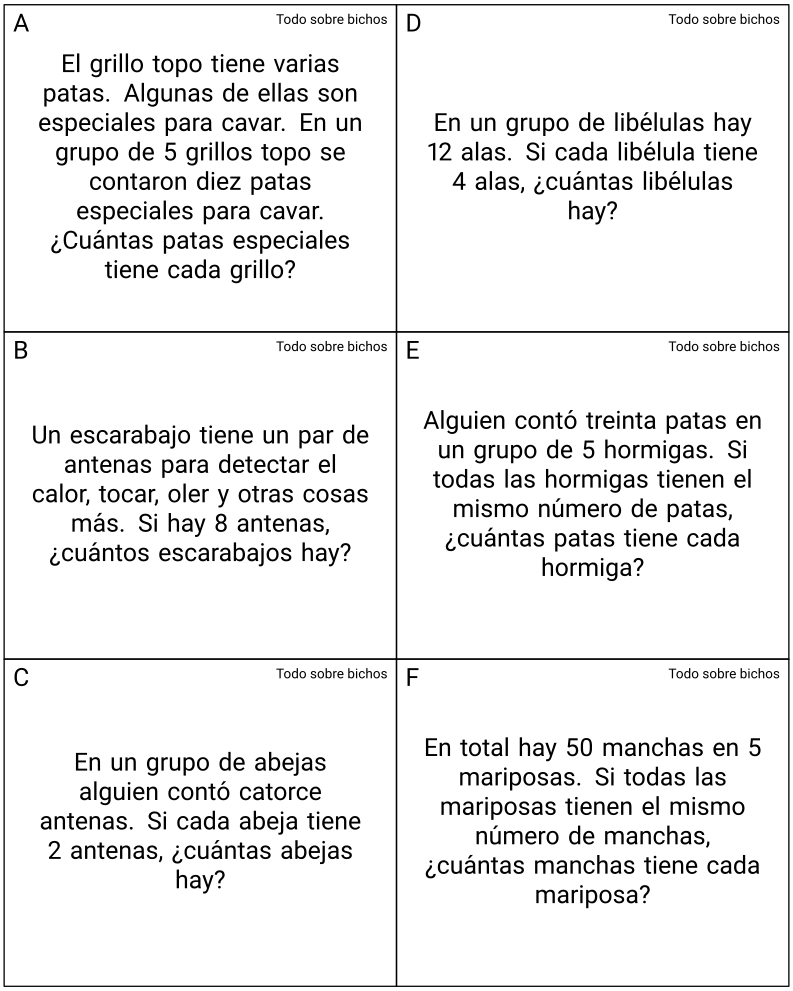
\includegraphics[max width=\linewidth, center]{external/tikz-source/todoSobreBichos-tarjetas.pdf}
% \end{image}%
% \cleardoublepage
\end{subsubsectionptx}
\end{cutoutpage}
%
%
\typeout{************************************************}
\typeout{Preguntas de comprensión  Actividad de cierre}
\typeout{************************************************}
%
\begin{reading-questions-subsubsection}{Preguntas de comprensión}{Actividad de cierre}{}{Actividad de cierre}{}{}{lec-escribamosExpresionesDivision-cool}
%
\end{reading-questions-subsubsection}
\end{subsectionptx}
%
%
\typeout{************************************************}
\typeout{Ejercicios  Problemas de práctica de la sección A}
\typeout{************************************************}
%
\begin{exercises-subsection}{Ejercicios}{Problemas de práctica de la sección A}{}{Problemas de práctica}{}{}{gra3-uni4-secA-ProblemasPractica}
%
%
%
%
%
%
%
%
%
%
%
%
\end{exercises-subsection}
\end{sectionptx}
%
%
\typeout{************************************************}
\typeout{Sección  Sección B -~Relacionemos la multiplicación y la división}
\typeout{************************************************}
%
\begin{sectionptx}{Sección}{Sección B -~Relacionemos la multiplicación y la división}{}{Sección B -~Relacionemos la multiplicación y la división}{}{}{gra3-uni4-secB}
%
%
\typeout{************************************************}
\typeout{Subsección  Lección 6 -~La división como un factor desconocido}
\typeout{************************************************}
%
\begin{subsectionptx}{Subsección}{Lección 6 -~La división como un factor desconocido}{}{Lección 6}{}{}{lec-divisionComoFactorDesconocido}
%
%
\typeout{************************************************}
\typeout{Subsubsección  Actividad 2}
\typeout{************************************************}
%
\begin{subsubsectionptx}{Subsubsección}{Actividad 2}{}{Actividad 2}{}{}{lec-divisionComoFactorDesconocido-act2}
\begin{activity}{Actividad}{En el mercado agrícola.}{act-enElMercadoAgricola}%
Completa cada fila. Prepárate para explicar tu razonamiento.%
\begin{image}{0}{1}{0}{}%
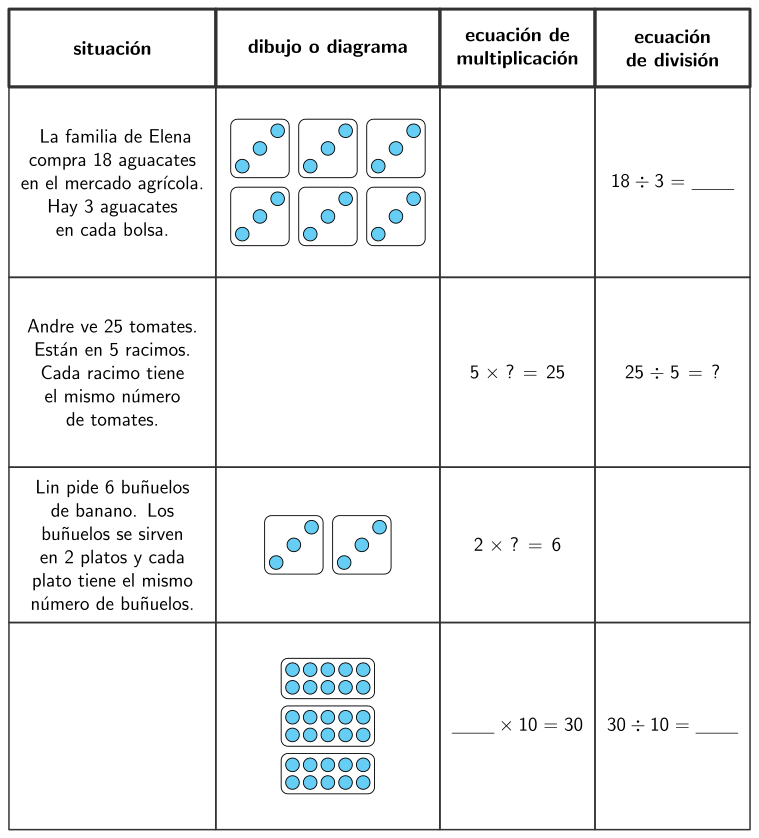
\includegraphics[max width=1.05\linewidth, center]{external/tikz-source/enElMercadoAgricola-blm-tab.pdf}
\end{image}%
\end{activity}%
\end{subsubsectionptx}
%
%
\typeout{************************************************}
\typeout{Preguntas de comprensión  Actividad de cierre}
\typeout{************************************************}
%
\begin{reading-questions-subsubsection}{Preguntas de comprensión}{Actividad de cierre}{}{Actividad de cierre}{}{}{lec-divisionComoFactorDesconocido-cool}
%
\end{reading-questions-subsubsection}
\end{subsectionptx}
%
%
\typeout{************************************************}
\typeout{Subsección  Lección 7 -~Relacionemos multiplicación y división}
\typeout{************************************************}
%
\begin{subsectionptx}{Subsección}{Lección 7 -~Relacionemos multiplicación y división}{}{Lección 7}{}{}{lec-relacionarMultiplicacionYDivision}
%
%
\typeout{************************************************}
\typeout{Subsubsección  Actividad 1}
\typeout{************************************************}
%
% \cleardoublepage
\begin{subsubsectionptx}{Subsubsección}{Actividad 1}{}{Actividad 1}{}{}{lec-relacionarMultiplicacionYDivision-act1}
\begin{activity}{Actividad}{Mesa redonda de división.}{act-mesaRedondaDeDivision}%
% En la siguiente tabla hay 4 recuadros. Tu profesor te pedirá que dibujes o escribas algo en cada uno.%
% \par
% Después de trabajar en cada recuadro, haz una pausa y espera que el profesor te dé las instrucciones para el siguiente recuadro.%
% %
% \begin{enumerate}
% \item{}Dibuja grupos iguales en el recuadro 1 de tu hoja de registro.%
% \item{}En el recuadro 2 de la hoja que acabaste de recibir, escribe una descripción de una situación de división que corresponda al dibujo.%
% \item{}En el recuadro 3 de la hoja que acabas de recibir, escribe una ecuación de multiplicación que corresponda al dibujo y a la situación de división. Usa un símbolo para representar la cantidad desconocida.%
% \item{}En el recuadro 4 de la hoja que acabas de recibir, escribe una ecuación de división que corresponda al dibujo, a la situación de división y a la ecuación de multiplicación. Usa un símbolo para representar la cantidad desconocida.%
% \end{enumerate}
\begin{image}{0}{1}{0}{}%
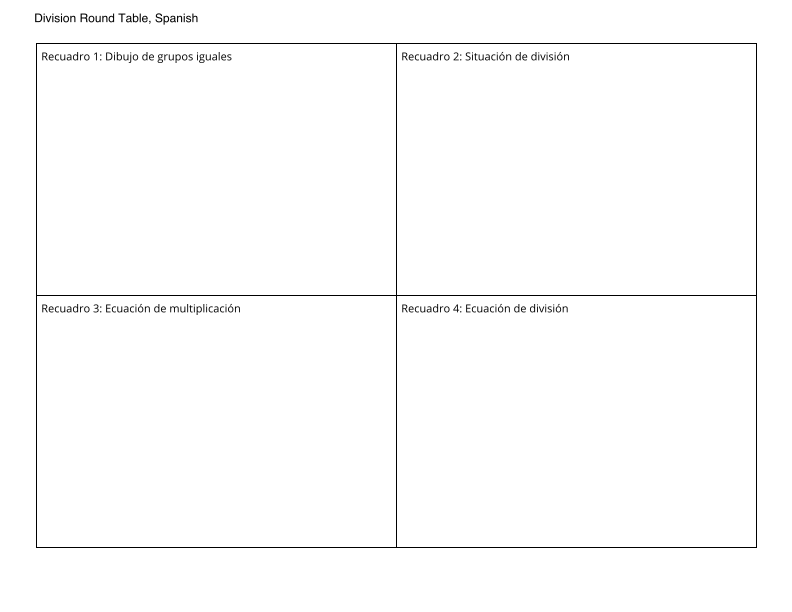
\includegraphics[trim=20 20 20 30, clip, width=1.3\linewidth,angle=90,origin=c]{external/blm/pdf-source/mesa-redonda-de-division.pdf}
\end{image}%
\end{activity}%
% \cleardoublepage
\end{subsubsectionptx}
%
%
\typeout{************************************************}
\typeout{Subsubsección  Actividad 2}
\typeout{************************************************}
%

%
%
\typeout{************************************************}
\typeout{Preguntas de comprensión  Actividad de cierre}
\typeout{************************************************}
%
\begin{reading-questions-subsubsection}{Preguntas de comprensión}{Actividad de cierre}{}{Actividad de cierre}{}{}{lec-relacionarMultiplicacionYDivision-cool}
%
\end{reading-questions-subsubsection}
\end{subsectionptx}
%
%
\typeout{************************************************}
\typeout{Subsección  Lección 8 -~Relacionemos cocientes con productos que nos sabemos}
\typeout{************************************************}
%
\begin{subsectionptx}{Subsección}{Lección 8 -~Relacionemos cocientes con productos que nos sabemos}{}{Lección 8}{}{}{lec-relCocientesProductos}
%
%
\typeout{************************************************}
\typeout{Subsubsección  Actividad 1}
\typeout{************************************************}
%
\begin{subsubsectionptx}{Subsubsección}{Actividad 1}{}{Actividad 1}{}{}{lec-relCocientesProductos-act1}
\begin{activity}{Actividad}{Clasificación de tarjetas: Multiplicación.}{act-clasificacionDeTarjetas-multiplicacion}%
Hazle preguntas a tu compañero sobre sus hechos de multiplicación. Clasifica los hechos de tu compañero en una de estas columnas:%
\begin{image}{0}{1}{0}{}%
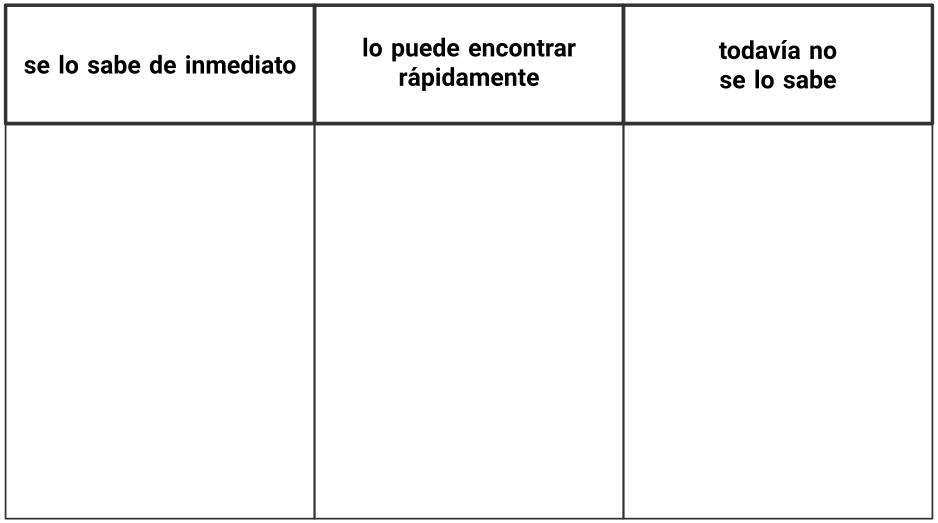
\includegraphics[max width=\linewidth, center]{external/tikz-source/clasificacionTarjetas-mult-paraBLM.pdf}
\end{image}%
Anota cinco expresiones de multiplicación que vas a practicar.%
%
\begin{enumerate}
\item{\vspace{0.5cm}}%
\item{\vspace{0.5cm}}%
\item{\vspace{0.5cm}}%
\item{\vspace{0.5cm}}%
\item{\vspace{0.5cm}}%
\end{enumerate}
\end{activity}%
\begin{cutoutpage}[Lección 8 - Clasificación de tarjetas: Multiplicación]
Tarjetas para recortar:
\par
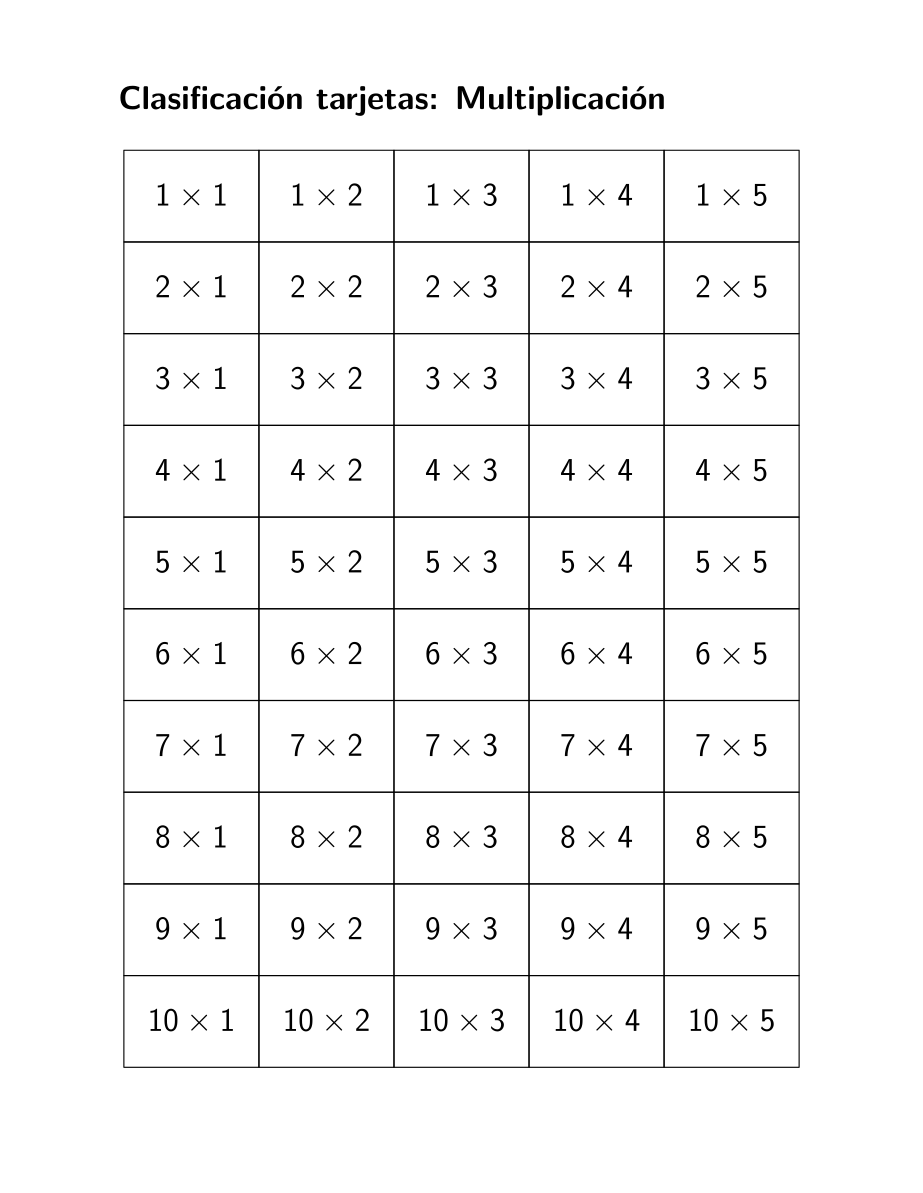
\includegraphics[page=1, trim=70 80 80 100,clip, width=1.05\linewidth]{external/blm/tikz-source/clasificacionTarjetas-multiplicacion-blm.pdf}

\cleardoublepage
Más tarjetas para recortar:
\par
\includegraphics[page=2, trim=70 80 80 100,clip, width=1.05\linewidth]{external/blm/tikz-source/clasificacionTarjetas-multiplicacion-blm.pdf}
\end{cutoutpage}

\end{subsubsectionptx}
%
%
\typeout{************************************************}
\typeout{Subsubsección  Actividad 2}
\typeout{************************************************}
%
\begin{subsubsectionptx}{Subsubsección}{Actividad 2}{}{Actividad 2}{}{}{lec-relCocientesProductos-act2}
\begin{activity}{Actividad}{Si sé que \textellipsis{}, entonces sé que \textellipsis{}.}{act-siSeQueEntoncesSeQue}%
Si sé que \(4 \times 5 = 20\), entonces sé que \fillintext{10}.%
%
\begin{enumerate}
\item{}Coloquen las tarjetas de hechos de multiplicación en un montón, boca abajo.%
\item{}Por turnos, tomen una tarjeta de hechos de multiplicación.%
\item{}Usen el hecho de multiplicación de la tarjeta para escribir una ecuación de multiplicación en la columna “Si sé que \textellipsis{}”%
\item{}Después, anoten las ecuaciones de división relacionadas en la columna “Entonces sé que   \textellipsis{}”%
\end{enumerate}
\begin{image}{0}{1}{0}{}%
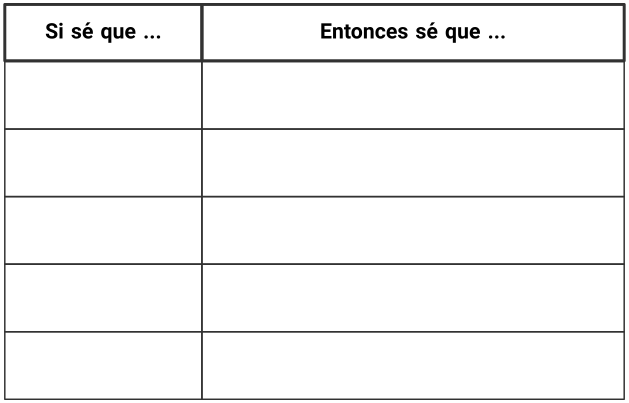
\includegraphics[max width=\linewidth, center]{external/tikz-source/siSeQueEntoncesSeQue-tab-libroTrabajo.pdf}
\end{image}%
\end{activity}%
\end{subsubsectionptx}
%
%
\typeout{************************************************}
\typeout{Preguntas de comprensión  Actividad de cierre}
\typeout{************************************************}
%
\begin{reading-questions-subsubsection}{Preguntas de comprensión}{Actividad de cierre}{}{Actividad de cierre}{}{}{lec-relCocientesProductos-cool}
%
\end{reading-questions-subsubsection}
\end{subsectionptx}
%
%
\typeout{************************************************}
\typeout{Subsección  Lección 9 -~Patrones en la tabla de multiplicar}
\typeout{************************************************}
%
\begin{subsectionptx}{Subsección}{Lección 9 -~Patrones en la tabla de multiplicar}{}{Lección 9}{}{}{lec-patronesTablaMultiplicar}
%
%
\typeout{************************************************}
\typeout{Subsubsección  Actividad 1}
\typeout{************************************************}
%

%
%
\typeout{************************************************}
\typeout{Subsubsección  Actividad 2}
\typeout{************************************************}
%
\clearpage
\begin{subsubsectionptx}{Subsubsección}{Actividad 2}{}{Actividad 2}{}{}{lec-patronesTablaMultiplicar-act2}
\begin{activity}{Actividad}{Si sé que \textellipsis{}, entonces sé que \textellipsis{}: Multiplicación.}{act-siSeQueEntoncesSeQueMult}%
%
\begin{enumerate}
\item{}En cada fila, escribe al menos dos hechos de multiplicación que puedes descifrar porque conoces el hecho de multiplicación dado en la columna de la izquierda. Prepárate para compartir tu razonamiento.%
\begin{image}{0}{1}{0}{}%
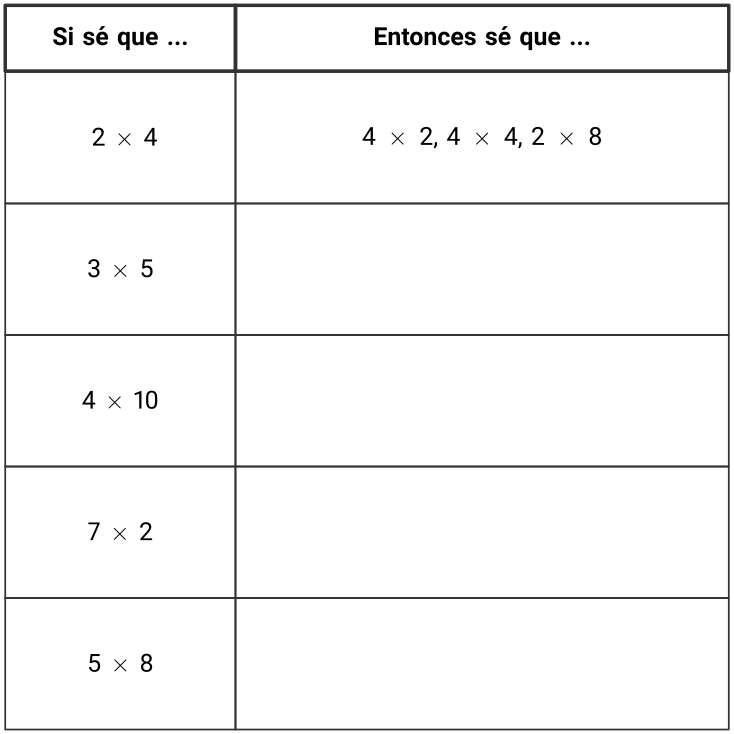
\includegraphics[max width=\linewidth, center]{external/tikz-source/siSeQueEntoncesSeQueMult-BLM-tab.pdf}
\end{image}%
\item{}Si te queda tiempo, completa el resto de la tabla de multiplicar. Usa los hechos de multiplicación que conoces para encontrar aquellos que no conoces.%
\end{enumerate}
\end{activity}%
\end{subsubsectionptx}
%
%
\typeout{************************************************}
\typeout{Preguntas de comprensión  Actividad de cierre}
\typeout{************************************************}
%
\begin{reading-questions-subsubsection}{Preguntas de comprensión}{Actividad de cierre}{}{Actividad de cierre}{}{}{lec-patronesTablaMultiplicar-cool}
%
\end{reading-questions-subsubsection}
\end{subsectionptx}
%
%
\typeout{************************************************}
\typeout{Subsección  Lección 10 -~Exploremos estrategias de multiplicación con rectángulos}
\typeout{************************************************}
%
\begin{subsectionptx}{Subsección}{Lección 10 -~Exploremos estrategias de multiplicación con rectángulos}{}{Lección 10}{}{}{lec-estrategiasMultConRectangulos}
%
%
\typeout{************************************************}
\typeout{Subsubsección  Actividad 1}
\typeout{************************************************}
%
\clearpage
\begin{subsubsectionptx}{Subsubsección}{Actividad 1}{}{Actividad 1}{}{}{lec-estrategiasMultConRectangulos-act1}
\begin{activity}{Actividad}{De diagramas a expresiones.}{act-deDiagramasAExpresiones}%
%
\begin{enumerate}
\item[2.] Este es otro rectángulo.%
\begin{image}{0}{1}{0}{}%
\includegraphics[max width=\linewidth, center]{external/svg-source/tikz-file-153048.pdf}
\end{image}%
Podemos encontrar su área hallando \(4 \times 9\).%
%
\begin{enumerate}
\item{}Marca o colorea el rectángulo de una manera que te ayude a encontrar su área.%
\item{}Escribe una o más expresiones que representen lo que hiciste en el diagrama y muestra cómo encontraste el área.%
% \begin{image}{0}{1}{0}{}%
% 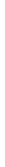
\includegraphics[max width=\linewidth, center]{external/whitespace-tikz/4cm.pdf}
% \end{image}%
\end{enumerate}
\end{enumerate}
\end{activity}%
\end{subsubsectionptx}
%
%
\typeout{************************************************}
\typeout{Subsubsección  Actividad 2}
\typeout{************************************************}
%
\begin{subsubsectionptx}{Subsubsección}{Actividad 2}{}{Actividad 2}{}{}{lec-estrategiasMultConRectangulos-act2}
\begin{activity}{Actividad}{De expresiones a diagramas.}{act-deExpresionesADiagramas}%
\begin{sidebyside}{3}{0.0166666666666667}{0.0166666666666667}{0.0333333333333333}%
\begin{sbspanel}{0.3}%
Noah%
\par
\includegraphics[max width=\linewidth, center]{external/svg-source/tikz-file-153051.pdf}
%
\begin{equation*}
(5\times 3)+(2 \times 3)
\end{equation*}
%
\end{sbspanel}%
\begin{sbspanel}{0.3}%
Priya%
\par
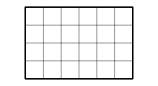
\includegraphics[max width=\linewidth, center]{external/svg-source/tikz-file-153053.pdf}
%
\begin{equation*}
2 \times (2 \times 6)
\end{equation*}
%
\end{sbspanel}%
\begin{sbspanel}{0.3}%
Tyler%
\par
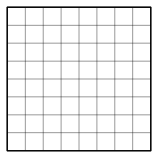
\includegraphics[max width=\linewidth, center]{external/svg-source/tikz-file-153054.pdf}
%
\begin{equation*}
(5 \times 8) + (3 \times 8)
\end{equation*}
%
\end{sbspanel}%
\end{sidebyside}%
\par
En cada rectángulo:%
%
\begin{enumerate}
\item{}Escribe los dos factores que se pueden multiplicar para encontrar su área.%
\item{}Marca o colorea cada rectángulo para mostrar la manera en la que cada estudiante vio el área. Prepárate para explicar tu razonamiento.%
\begin{image}{0}{1}{0}{}%
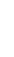
\includegraphics[max width=\linewidth, center]{external/whitespace-tikz/1cm.pdf}
\end{image}%
\end{enumerate}
\end{activity}%
\end{subsubsectionptx}
%
%
\typeout{************************************************}
\typeout{Preguntas de comprensión  Actividad de cierre}
\typeout{************************************************}
%
\begin{reading-questions-subsubsection}{Preguntas de comprensión}{Actividad de cierre}{}{Actividad de cierre}{}{}{lec-estrategiasMultConRectangulos-cool}
%
\end{reading-questions-subsubsection}
\end{subsectionptx}
%
%
\typeout{************************************************}
\typeout{Subsección  Lección 11 -~Estrategias de multiplicación para rectángulos sin cuadrícula}
\typeout{************************************************}
%
\begin{subsectionptx}{Subsección}{Lección 11 -~Estrategias de multiplicación para rectángulos sin cuadrícula}{}{Lección 11}{}{}{lec-estrategiasMultRectangulosSinCuadricula}
%
%
\typeout{************************************************}
\typeout{Subsubsección  Actividad 1}
\typeout{************************************************}
%
\begin{subsubsectionptx}{Subsubsección}{Actividad 1}{}{Actividad 1}{}{}{gra3-uni4-secB-lec11-act1}
\begin{activity}{Actividad}{Marca y después expresa.}{act-marcaDespuesExpresa}%
En cada caso:%
%
\begin{itemize}[label=\textbullet]
\item{}Marca o colorea cada rectángulo para mostrar una estrategia que ayude a encontrar su área.%
\item{}Escribe una o más expresiones que representen cómo encuentras el área.%
\end{itemize}
\begin{sidebyside}{3}{0}{0}{0}%
\begin{sbspanel}{0.391}%
A%
\par
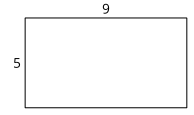
\includegraphics[max width=\linewidth, center]{external/svg-source/tikz-file-153084.pdf}
\end{sbspanel}%
\begin{sbspanel}{0.261}%
B%
\par
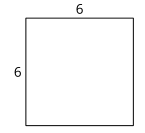
\includegraphics[max width=\linewidth, center]{external/svg-source/tikz-file-153085.pdf}
\end{sbspanel}%
\begin{sbspanel}{0.348}%
C%
\par
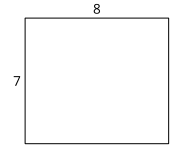
\includegraphics[max width=\linewidth, center]{external/svg-source/tikz-file-153086.pdf}
\end{sbspanel}%
\end{sidebyside}%
\begin{image}{0}{1}{0}{}%
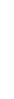
\includegraphics[max width=\linewidth, center]{external/whitespace-tikz/2cm.pdf}
\end{image}%
\end{activity}%
\end{subsubsectionptx}
%
%
\typeout{************************************************}
\typeout{Subsubsección  Actividad 2}
\typeout{************************************************}
%
\begin{subsubsectionptx}{Subsubsección}{Actividad 2}{}{Actividad 2}{}{}{gra3-uni4-secB-lec11-act2}
\begin{activity}{Actividad}{Clasificación de tarjetas: Expresiones diferentes, mismo rectángulo.}{act-clasificacionDeTarjetas-expresionesMultiplicacionRectangulos}%
Las tarjetas para recortar tienen expresiones que representan áreas de rectángulos.%
\par
Clasifica las expresiones en grupos de manera que las expresiones de cada grupo representen el área del mismo rectángulo. Prepárate para explicar tu razonamiento.%
\par
Si te ayuda, puedes dibujar rectángulos.%
\end{activity}%
% \cleardoublepage
\begin{cutoutpage}[Lección 11 -- Clasificación de tarjetas: Expresiones diferentes, mismo rectángulo]
Tarjetas para recortar:
\begin{image}{0}{1}{0}{}%
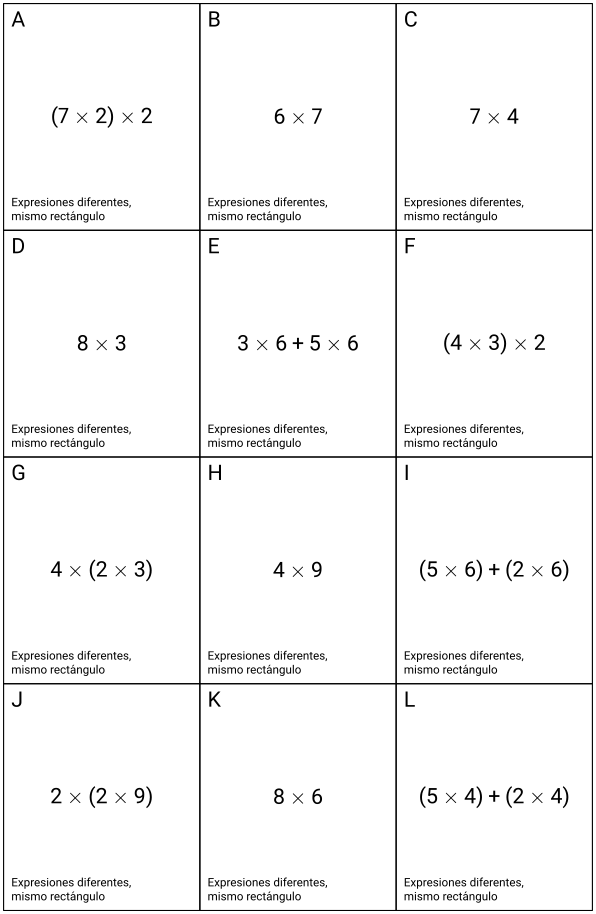
\includegraphics[max width=\linewidth, center]{external/blm/tikz-source/clasificacionTarjetas-expresionesDiferentesMismoRect-tarjetas.pdf}
\end{image}
\end{cutoutpage}
% \cleardoublepage
\end{subsubsectionptx}
%
%
\typeout{************************************************}
\typeout{Preguntas de comprensión  Actividad de cierre}
\typeout{************************************************}
%
\begin{reading-questions-subsubsection}{Preguntas de comprensión}{Actividad de cierre}{}{Actividad de cierre}{}{}{gra3-uni4-secB-lec11-cool}
%
\end{reading-questions-subsubsection}
\end{subsectionptx}
%
%
\typeout{************************************************}
\typeout{Ejercicios  Problemas de práctica de la sección B}
\typeout{************************************************}
%
\begin{exercises-subsection}{Ejercicios}{Problemas de práctica de la sección B}{}{Problemas de práctica}{}{}{gra3-uni4-secB-ProblemasPractica}
%
%
%
%
%
%
%
\end{exercises-subsection}
\end{sectionptx}
%
%
\typeout{************************************************}
\typeout{Sección  Sección C -~Multipliquemos números más grandes}
\typeout{************************************************}
%
\begin{sectionptx}{Sección}{Sección C -~Multipliquemos números más grandes}{}{Sección C -~Multipliquemos números más grandes}{}{}{gra3-uni4-secC}
%
%
\typeout{************************************************}
\typeout{Subsección  Lección 12 -~Multipliquemos múltiplos de diez}
\typeout{************************************************}
%
\begin{subsectionptx}{Subsección}{Lección 12 -~Multipliquemos múltiplos de diez}{}{Lección 12}{}{}{lec-multiplicarMultiplos10}
%
%
\typeout{************************************************}
\typeout{Subsubsección  Actividad 1}
\typeout{************************************************}
%
\begin{subsubsectionptx}{Subsubsección}{Actividad 1}{}{Actividad 1}{}{}{lec-multiplicarMultiplos10-act1}
\begin{activity}{Actividad}{Una gran cantidad de dólares.}{act-granCantidadDolares}%
Seis amigos juegan un juego de mesa en el que se usa dinero de juguete. Hay billetes de papel de \textdollar{}5, \textdollar{}10, \textdollar{}20, \textdollar{}50 y de \textdollar{}100.%
%
\begin{enumerate}
\item{}Cada jugador recibió \textdollar{}100 para empezar. ¿Cuáles de los siguientes podrían ser los billetes que recibió cada jugador?%
\par
Escribe una expresión que represente los billetes de juguete y escribe la cantidad de dólares.%
\begin{image}{0}{1}{0}{}%
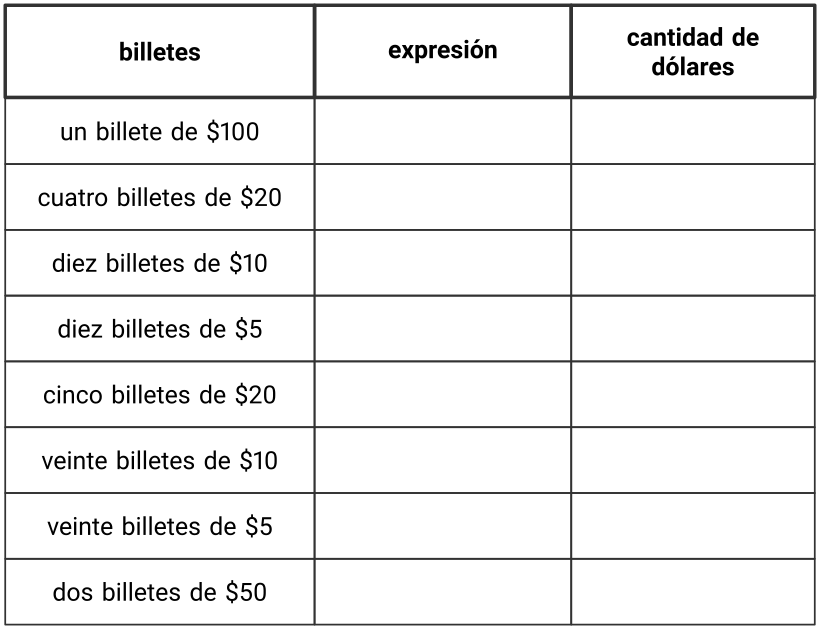
\includegraphics[max width=\linewidth, center]{external/tikz-source/unaGranCantidadDeDolares-tab1.pdf}
\end{image}%
\item{}En un momento del juego, Noah tuvo que pagarle a Lin \textdollar{}150. Él le dio esa cantidad usando billetes del mismo tipo.%
%
\begin{enumerate}
\item{}¿Cuáles y cuántos billetes podría haber usado Noah para completar \textdollar{}150? Nombra todas las posibilidades.%
\begin{image}{0}{1}{0}{}%
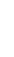
\includegraphics[max width=\linewidth, center]{external/whitespace-tikz/1cm.pdf}
\end{image}%
\item{}Escribe una expresión para cada forma en la que Noah podría haberle pagado a Lin.%
% \begin{image}{0}{1}{0}{}%
% 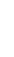
\includegraphics[max width=\linewidth, center]{external/whitespace-tikz/1cm.pdf}
% \end{image}%
\end{enumerate}
\clearpage
\item{}La tabla muestra lo que tenían los jugadores al final del juego. Gana la persona que tenga la mayor cantidad de dinero. ¿Quién ganó el juego?%
\par
Escribe una expresión que represente los billetes que tiene cada persona y escribe la cantidad de dólares.%
\begin{image}{0}{1}{0}{}%
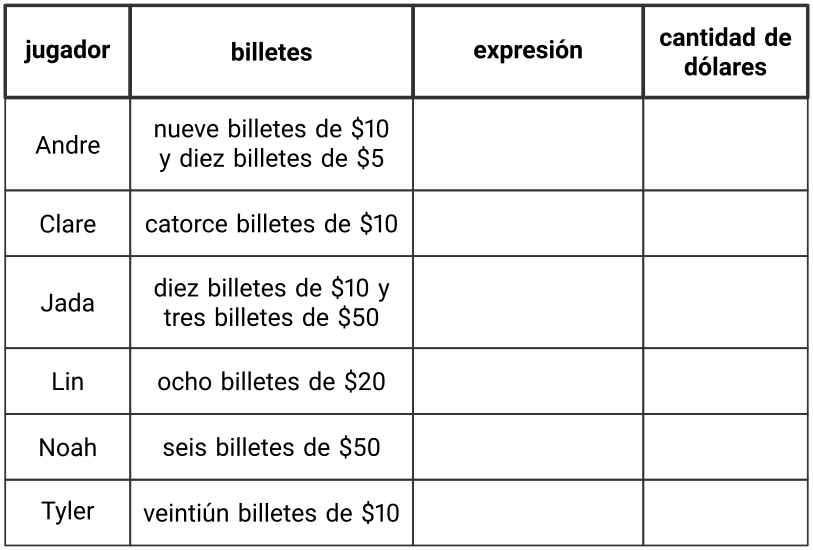
\includegraphics[max width=\linewidth, center]{external/tikz-source/unaGranCantidadDeDolares-tab2.pdf}
\end{image}%
\end{enumerate}
\end{activity}%
\end{subsubsectionptx}
%
%
\typeout{************************************************}
\typeout{Preguntas de comprensión  Actividad de cierre}
\typeout{************************************************}
%
\begin{reading-questions-subsubsection}{Preguntas de comprensión}{Actividad de cierre}{}{Actividad de cierre}{}{}{lec-multiplicarMultiplos10-cool}
%
\end{reading-questions-subsubsection}
\end{subsectionptx}
%
%
\typeout{************************************************}
\typeout{Subsección  Lección 13 -~Resolvamos problemas de grupos iguales}
\typeout{************************************************}
%
\begin{subsectionptx}{Subsección}{Lección 13 -~Resolvamos problemas de grupos iguales}{}{Lección 13}{}{}{lec-problemasMult11a19}
%
%
%
%
\typeout{************************************************}
\typeout{Preguntas de comprensión  Actividad de cierre}
\typeout{************************************************}
%
\begin{reading-questions-subsubsection}{Preguntas de comprensión}{Actividad de cierre}{}{Actividad de cierre}{}{}{lec-problemasMult11a19-cool}
%
\end{reading-questions-subsubsection}
\end{subsectionptx}
%
%
\typeout{************************************************}
\typeout{Subsección  Lección 14 -~Formas de representar la multiplicación de números del 11 al 19}
\typeout{************************************************}
%
\begin{subsectionptx}{Subsección}{Lección 14 -~Formas de representar la multiplicación de números del 11 al 19}{}{Lección 14}{}{}{lec-representarMultiplicacion11a19}
%
%
\typeout{************************************************}
\typeout{Preguntas de comprensión  Actividad de cierre}
\typeout{************************************************}
%
\begin{reading-questions-subsubsection-numberless}{Preguntas de comprensión}{Actividad de cierre}{}{Actividad de cierre}{}{}{lec-representarMultiplicacion11a19-cool}
%
\end{reading-questions-subsubsection-numberless}
\end{subsectionptx}
%
%
\typeout{************************************************}
\typeout{Subsección  Lección 15 -~Grupos iguales, números más grandes}
\typeout{************************************************}
%
\begin{subsectionptx}{Subsección}{Lección 15 -~Grupos iguales, números más grandes}{}{Lección 15}{}{}{lec-problemasMult11a19MasGrandes}
%
%
\typeout{************************************************}
\typeout{Preguntas de comprensión  Actividad de cierre}
\typeout{************************************************}
%
\begin{reading-questions-subsubsection-numberless}{Preguntas de comprensión}{Actividad de cierre}{}{Actividad de cierre}{}{}{lec-problemasMult11a19MasGrandes-cool}
%
\end{reading-questions-subsubsection-numberless}
\end{subsectionptx}
%
%
\typeout{************************************************}
\typeout{Subsección  Lección 16 -~Multipliquemos números más grandes que 20}
\typeout{************************************************}
%
\begin{subsectionptx}{Subsección}{Lección 16 -~Multipliquemos números más grandes que 20}{}{Lección 16}{}{}{lec-multiplicarNumsMayoresA20}
%
%
\typeout{************************************************}
\typeout{Subsubsección  Actividad 3}
\typeout{************************************************}
%
\clearpage
\begin{subsubsectionptx}{Subsubsección}{Actividad 3}{}{Actividad 3}{}{}{lec-multiplicarNumsMayoresA20-act3}
\begin{activity}{Actividad}{Juguemos “Cerca de 100, multiplicación” (opcional).}{act-juegoCerca100Multiplicacion}%
Tarjetas para recortar en las siguiente páginas.%
% %
% \begin{enumerate}
% \item{}Pon las tarjetas boca abajo.%
% \item{}Cada jugador toma 4 tarjetas.%
% \item{}Cada jugador escoge 2 de sus tarjetas para completar la expresión y hacer que el valor esté lo más cerca posible de 100. Escribe los 2 dígitos y el producto.%
% \item{}El jugador que esté más cerca de 100, gana esa ronda.%
% \item{}Juega 5 rondas. El jugador que gane la mayoría de rondas, gana la partida.%
% \end{enumerate}
\begin{sidebyside}{2}{0}{0}{0.1}%
\begin{sbspanel}{0.45}%
\alert{Partida 1}%
\end{sbspanel}%
\begin{sbspanel}{0.45}%
\par
\alert{Partida 2}%
\end{sbspanel}%
\end{sidebyside}%
\begin{sidebyside}{2}{0}{0}{0.1}%
\begin{sbspanel}{0.45}%
Ronda 1%
\par
%
\begin{equation*}
\boxed{\phantom{\frac{00}{00}}} \times 1 \ \boxed{\phantom{\frac{00}{00}}}= \underline{\hspace{1cm}}
\end{equation*}
%
\end{sbspanel}%
\begin{sbspanel}{0.45}%
Ronda 1%
\par
%
\begin{equation*}
\boxed{\phantom{\frac{00}{00}}} \times 2 \ \boxed{\phantom{\frac{00}{00}}}= \underline{\hspace{1cm}}
\end{equation*}
%
\end{sbspanel}%
\end{sidebyside}%
\begin{sidebyside}{2}{0}{0}{0.1}%
\begin{sbspanel}{0.45}%
Ronda 2%
\par
%
\begin{equation*}
\boxed{\phantom{\frac{00}{00}}} \times 1 \ \boxed{\phantom{\frac{00}{00}}}= \underline{\hspace{1cm}}
\end{equation*}
%
\end{sbspanel}%
\begin{sbspanel}{0.45}%
Ronda 2%
\par
%
\begin{equation*}
\boxed{\phantom{\frac{00}{00}}} \times 2 \ \boxed{\phantom{\frac{00}{00}}}= \underline{\hspace{1cm}}
\end{equation*}
%
\end{sbspanel}%
\end{sidebyside}%
\begin{sidebyside}{2}{0}{0}{0.1}%
\begin{sbspanel}{0.45}%
Ronda 3%
\par
%
\begin{equation*}
\boxed{\phantom{\frac{00}{00}}} \times 1 \ \boxed{\phantom{\frac{00}{00}}}= \underline{\hspace{1cm}}
\end{equation*}
%
\end{sbspanel}%
\begin{sbspanel}{0.45}%
Ronda 3%
\par
%
\begin{equation*}
\boxed{\phantom{\frac{00}{00}}} \times 2 \ \boxed{\phantom{\frac{00}{00}}}= \underline{\hspace{1cm}}
\end{equation*}
%
\end{sbspanel}%
\end{sidebyside}%
\begin{sidebyside}{2}{0}{0}{0.1}%
\begin{sbspanel}{0.45}%
Ronda 4%
\par
%
\begin{equation*}
\boxed{\phantom{\frac{00}{00}}} \times 1 \ \boxed{\phantom{\frac{00}{00}}}= \underline{\hspace{1cm}}
\end{equation*}
%
\end{sbspanel}%
\begin{sbspanel}{0.45}%
Ronda 4%
\par
%
\begin{equation*}
\boxed{\phantom{\frac{00}{00}}} \times 2 \ \boxed{\phantom{\frac{00}{00}}}= \underline{\hspace{1cm}}
\end{equation*}
%
\end{sbspanel}%
\end{sidebyside}%
\begin{sidebyside}{2}{0}{0}{0.1}%
\begin{sbspanel}{0.45}%
Ronda 5%
\par
%
\begin{equation*}
\boxed{\phantom{\frac{00}{00}}} \times 1 \ \boxed{\phantom{\frac{00}{00}}}= \underline{\hspace{1cm}}
\end{equation*}
%
\end{sbspanel}%
\begin{sbspanel}{0.45}%
Ronda 5%
\par
%
\begin{equation*}
\boxed{\phantom{\frac{00}{00}}} \times 2 \ \boxed{\phantom{\frac{00}{00}}}= \underline{\hspace{1cm}}
\end{equation*}
%
\end{sbspanel}%
\end{sidebyside}%
%
\end{activity}%
% \cleardoublepage
\begin{cutoutpage}[Lección 16 -- Juguemos “Cerca de 100, multiplicación” (opcional)]
Tarjetas para recortar:
\begin{image}{0}{1}{0}{}%
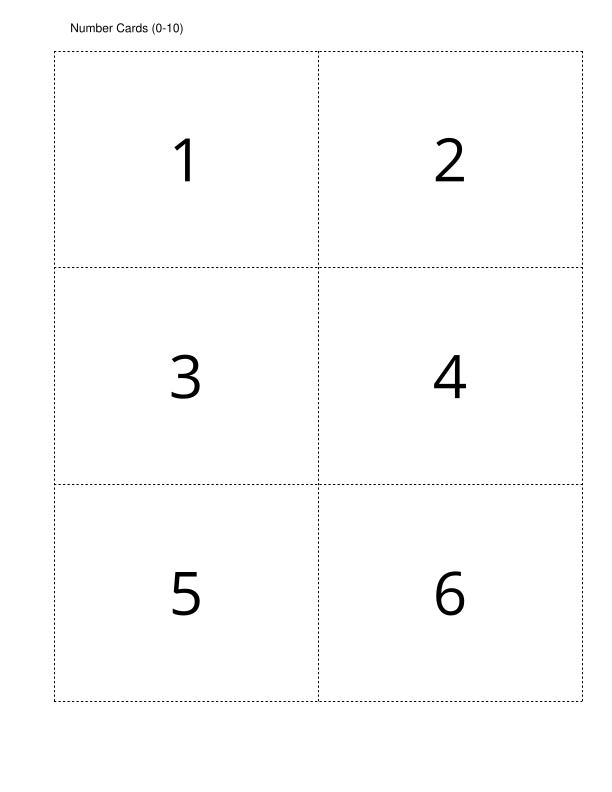
\includegraphics[page=1, rotate=90, scale=0.55, trim=40 40 20 40, clip, center] {external/blm/pdf-source/tarjetasDeDigitos.pdf}
\end{image}%
\begin{image}{0}{1}{0}{}%
\includegraphics[page=2, rotate=90, scale=0.55, trim=40 40 20 40, clip, center] {external/blm/pdf-source/tarjetasDeDigitos.pdf}
\end{image}%
\cleardoublepage
Tarjetas para recortar:
\begin{image}{0}{1}{0}{}%
\includegraphics[page=3, rotate=90, scale=0.55, trim=40 40 20 40, clip, center] {external/blm/pdf-source/tarjetasDeDigitos.pdf}
\end{image}%
\begin{image}{0}{1}{0}{}%
\includegraphics[page=4, rotate=90, scale=0.55, trim=40 40 20 40, clip, center] {external/blm/pdf-source/tarjetasDeDigitos.pdf}
\end{image}
\end{cutoutpage}
% \cleardoublepage
\end{subsubsectionptx}
%
%
\typeout{************************************************}
\typeout{Preguntas de comprensión  Actividad de cierre}
\typeout{************************************************}
%
\begin{reading-questions-subsubsection}{Preguntas de comprensión}{Actividad de cierre}{}{Actividad de cierre}{}{}{lec-multiplicarNumsMayoresA20-cool}
%
\end{reading-questions-subsubsection}
\end{subsectionptx}
%
%
\typeout{************************************************}
\typeout{Subsección  Lección 17 -~Usemos las cuatro operaciones para resolver problemas}
\typeout{************************************************}
%
\begin{subsectionptx}{Subsección}{Lección 17 -~Usemos las cuatro operaciones para resolver problemas}{}{Lección 17}{}{}{lec-problemasCuatroOperaciones}
%
%
\typeout{************************************************}
\typeout{Preguntas de comprensión  Actividad de cierre}
\typeout{************************************************}
%
\begin{reading-questions-subsubsection-numberless}{Preguntas de comprensión}{Actividad de cierre}{}{Actividad de cierre}{}{}{lec-problemasCuatroOperaciones-cool}
%
\end{reading-questions-subsubsection-numberless}
\end{subsectionptx}
%
%
\typeout{************************************************}
\typeout{Ejercicios  Problemas de práctica de la sección C}
\typeout{************************************************}
%
\begin{exercises-subsection}{Ejercicios}{Problemas de práctica de la sección C}{}{Problemas de práctica}{}{}{gra3-uni4-secC-ProblemasPractica}
%
%

\end{exercises-subsection}
\end{sectionptx}
%
%
\typeout{************************************************}
\typeout{Sección  Sección D -~Dividamos números más grandes}
\typeout{************************************************}
%
\begin{sectionptx}{Sección}{Sección D -~Dividamos números más grandes}{}{Sección D -~Dividamos números más grandes}{}{}{gra3-uni4-secD}
%
%
\typeout{************************************************}
\typeout{Subsección  Lección 18 -~Números más grandes en grupos iguales}
\typeout{************************************************}
%
\begin{subsectionptx}{Subsección}{Lección 18 -~Números más grandes en grupos iguales}{}{Lección 18}{}{}{lec-gruposIgualesMasGrandes}
%
%
\typeout{************************************************}
\typeout{Preguntas de comprensión  Actividad de cierre}
\typeout{************************************************}
%
\begin{reading-questions-subsubsection-numberless}{Preguntas de comprensión}{Actividad de cierre}{}{Actividad de cierre}{}{}{lec-gruposIgualesMasGrandes-cool}
%
\end{reading-questions-subsubsection-numberless}
\end{subsectionptx}
%
%
\typeout{************************************************}
\typeout{Subsección  Lección 19 -~Formas de dividir números más grandes}
\typeout{************************************************}
%
\begin{subsectionptx}{Subsección}{Lección 19 -~Formas de dividir números más grandes}{}{Lección 19}{}{}{lec-formasDividirNumerosMasGrandes}
%
%
\typeout{************************************************}
\typeout{Preguntas de comprensión  Actividad de cierre}
\typeout{************************************************}
%
\begin{reading-questions-subsubsection-numberless}{Preguntas de comprensión}{Actividad de cierre}{}{Actividad de cierre}{}{}{lec-formasDividirNumerosMasGrandes-cool}
%
\end{reading-questions-subsubsection-numberless}
\end{subsectionptx}
%
%
\typeout{************************************************}
\typeout{Subsección  Lección 20 -~Estrategias para dividir}
\typeout{************************************************}
%
\begin{subsectionptx}{Subsección}{Lección 20 -~Estrategias para dividir}{}{Lección 20}{}{}{lec-estrategiasDividir}
%
%
\typeout{************************************************}
\typeout{Subsubsección  Actividad 3}
\typeout{************************************************}
%
% \cleardoublepage
\begin{cutoutpage}
\begin{subsubsectionptx}{Subsubsección}{Actividad 3}{}{Actividad 3}{}{}{lec-estrategiasDividir-act3}
\begin{activity}{Actividad}{“Compara: Divide hasta 100” [OPCIONAL].}{act-comparaDivideHasta100}%
Tarjetas para recortar%
\end{activity}%
% \begin{image}{0}{1}{0}{}%
\includegraphics[max width=0.9\linewidth, center]{external/blm/tikz-source/act-comparaDivideHasta100-tarjetas-grandes1.pdf}
% \end{image}%
\cleardoublepage
% \begin{image}{0}{1}{0}{}%
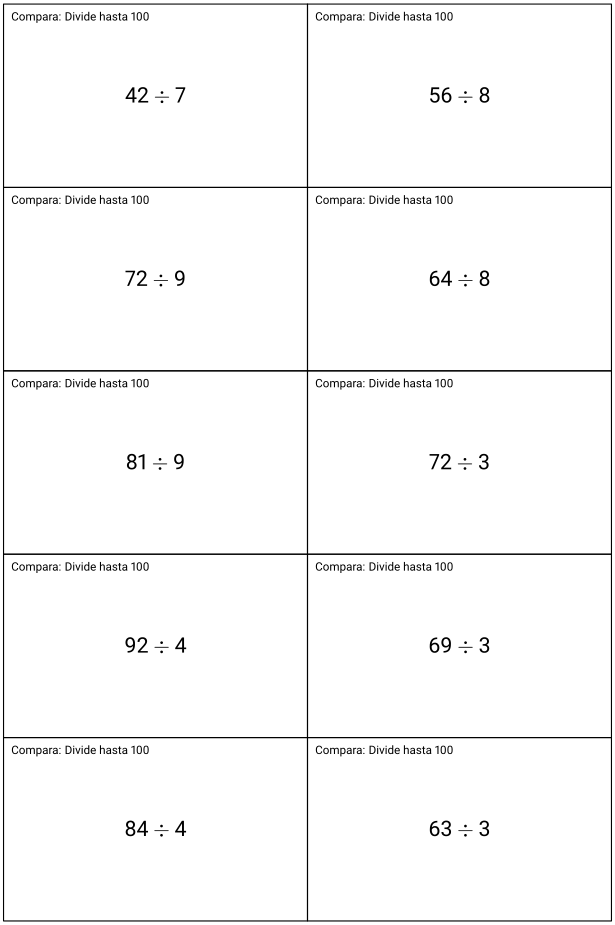
\includegraphics[max width=0.9\linewidth, center]{external/blm/tikz-source/act-comparaDivideHasta100-tarjetas-grandes2.pdf}
% \end{image}%
% \cleardoublepage
\end{subsubsectionptx}
\end{cutoutpage}
%
%
\typeout{************************************************}
\typeout{Preguntas de comprensión  Actividad de cierre}
\typeout{************************************************}
%
\begin{reading-questions-subsubsection}{Preguntas de comprensión}{Actividad de cierre}{}{Actividad de cierre}{}{}{lec-estrategiasDividir-cool}
%
\end{reading-questions-subsubsection}
\end{subsectionptx}
%
%
\typeout{************************************************}
\typeout{Subsección  Lección 21 -~Resolvamos problemas usando las cuatro operaciones}
\typeout{************************************************}
%
\begin{subsectionptx}{Subsección}{Lección 21 -~Resolvamos problemas usando las cuatro operaciones}{}{Lección 21}{}{}{lec-problemas4Operaciones}
%
%
\typeout{************************************************}
\typeout{Subsubsección  Actividad 1}
\typeout{************************************************}
%
\begin{subsubsectionptx}{Subsubsección}{Actividad 1}{}{Actividad 1}{}{}{lec-problemas4Operaciones-act1}
\begin{activity}{Actividad}{Una aventura con manzanas.}{act-unaAventuraConManzanas}%
\begin{sidebyside}{2}{0}{0}{0.1}%
\begin{sbspanel}{0.6}%
Un agricultor recogió algunas manzanas. Algunas de las manzanas están empacadas en cajas y algunas no.%
\end{sbspanel}%
\begin{sbspanel}{0.3}%
\includegraphics[max width=\linewidth, center]{external/png-source/3.4.D21.S_Sp.png}
\end{sbspanel}%
\end{sidebyside}%
\par
Escoge \(4\) números de la lista que describan correctamente la situación. Úsalos para llenar una fila de la tabla. Prepárate para explicar por qué tiene sentido juntar esos \(4\) números.%
\begin{image}{0}{1}{0}{}%
\includegraphics[max width=\linewidth, center]{external/svg-source/tikz-file-149345-scale13.pdf}
\end{image}%
\begin{image}{0}{1}{0}{}%
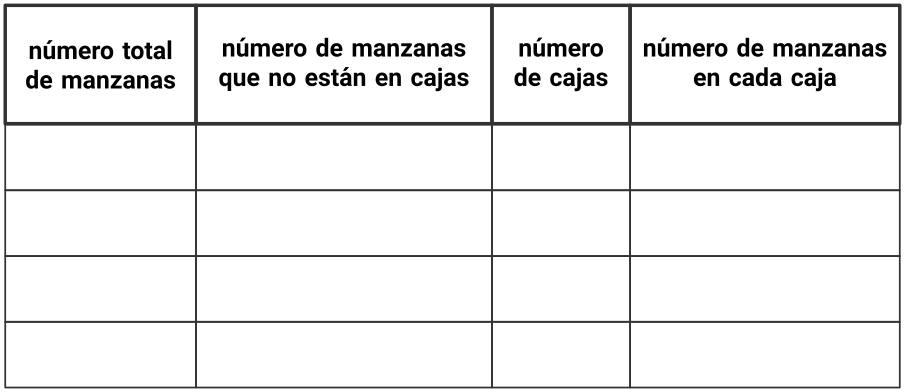
\includegraphics[max width=\linewidth, center]{external/tikz-source/3-4-21-act1-BLM-table.pdf}
\end{image}%
\end{activity}%
\end{subsubsectionptx}
%
%
\typeout{************************************************}
\typeout{Preguntas de comprensión  Actividad de cierre}
\typeout{************************************************}
%
\begin{reading-questions-subsubsection}{Preguntas de comprensión}{Actividad de cierre}{}{Actividad de cierre}{}{}{lec-problemas4Operaciones-cool}
%
\end{reading-questions-subsubsection}
\end{subsectionptx}
%
%
\typeout{************************************************}
\typeout{Subsección  Lección 22 -~La huerta comunitaria de la escuela}
\typeout{************************************************}
%
\begin{subsectionptx}{Subsección}{Lección 22 -~La huerta comunitaria de la escuela}{}{Lección 22}{}{}{lec-huertaComunitaria}
\end{subsectionptx}
%
%
\typeout{************************************************}
\typeout{Ejercicios  Problemas de práctica de la sección D}
\typeout{************************************************}
%
\begin{exercises-subsection}{Ejercicios}{Problemas de práctica de la sección D}{}{Problemas de práctica}{}{}{gra3-uni4-secD-ProblemasPractica}
%
% \vspace{2cm}
%
%
%
%
%
%
\end{exercises-subsection}
\end{sectionptx}
%
%
% \clearpage
\typeout{************************************************}
\typeout{Referencias  Atribuciones de imágenes}
\typeout{************************************************}
%
% \begin{references-section}{Referencias}{Atribuciones de imágenes}{}{Atribuciones de imágenes}{}{}{gra3-uni4-9}
% %
% \begin{itemize}[label=\textbullet]
% \item{}\hyperref[act-clasificacionDeTarjetas-todoSobreBichos]{Clasificación de tarjetas: Todo sobre bichos, p.\,\pageref{act-clasificacionDeTarjetas-todoSobreBichos}} Nicholas Caffarilla. CC-BY-SA 3.0. Wikipedia. \href{https://en.wikipedia.org/wiki/File:Insect_collage.png}{https:\slash{}\slash{}en.wikipedia.org}\footnote{\nolinkurl{en.wikipedia.org/wiki/File:Insect_collage.png}\label{gra3-uni4-9-2-4-3}}.%
% \end{itemize}
% Las imágenes sin atrubición las produjo LEMA \href{https://www.grupolema.org}{www.grupolema.org}\footnote{\nolinkurl{www.grupolema.org}\label{gra3-uni4-9-3-2}} específicamente para esta adaptación y se liberan con una licencia Creative Commons Attribution 4.0 International License (CC BY 4.0), o son © 2021 \href{https://curriculum.illustrativemathematics.org}{Illustrative Mathematics}\footnote{\nolinkurl{curriculum.illustrativemathematics.org}\label{gra3-uni4-9-3-4}} con una licencia Creative Commons Attribution 4.0 International License (CC BY 4.0) y se reproducen directamente de la versión en Español disponible en \href{https://im.kendallhunt.com/K5_ES/curriculum.html}{im.kendallhunt.com}\footnote{\nolinkurl{im.kendallhunt.com/K5_ES/curriculum.html}\label{gra3-uni4-9-3-6}}.%
% \end{references-section}
\end{document}
